\documentclass[10pt,twocolumn]{IEEEtran}

%% set page size to US letter
\special{papersize=8.5in,11in}
\setlength{\pdfpageheight}{\paperheight}
\setlength{\pdfpagewidth}{\paperwidth}

\DeclareMathAlphabet{\mathtsl}{OT1}{ptm}{m}{sl}
\RequirePackage{amssymb}
\usepackage{hyperref}
\usepackage{xspace}
\usepackage{algorithm}
\usepackage[noend]{algpseudocode}
\usepackage{amsbsy}
\usepackage{amsthm}
\usepackage{graphicx}
\usepackage{helvet}
\usepackage{enumerate}
\usepackage{amsmath}
\usepackage{amstext}
\usepackage{amsfonts}
\usepackage{graphicx}
\usepackage{multirow}
\usepackage{subfig}
\usepackage{comment}
\usepackage{cases}
\usepackage{xcolor}
\usepackage{epstopdf}
\usepackage[normalem]{ulem}
\usepackage{diagbox}
\usepackage{bm}

% \usepackage{titlesec}
% \titlespacing*{\section}{0pt}{1.1\baselineskip}{\baselineskip}

% \input{myformulae.tex}

% New command for the line spacing.
\newcommand{\ls}[1]
    {\dimen0=\fontdimen6\the\font
     \lineskip=#1\dimen0
     \advance\lineskip.5\fontdimen5\the\font
     \advance\lineskip-\dimen0
     \lineskiplimit=.9\lineskip
     \baselineskip=\lineskip
     \advance\baselineskip\dimen0
     \normallineskip\lineskip
     \normallineskiplimit\lineskiplimit
     \normalbaselineskip\baselineskip
     \ignorespaces
    }
% New command for the table bnotes.
\def\tabnote#1{{\small{#1}}}

\newcommand{\beqarr}{\begin{eqnarray}}
\newcommand{\eeqarr}{\end{eqnarray}}
\newcommand{\ov}{\bar}
\newcommand{\xor}{\bigoplus}
\newcommand{\Fm}{{\mathbb{F}}}
\newcommand{\myfontsize}{\fontsize{7}{9}\selectfont}
\newcommand{\Ftwo}{{\mathbb{F}}_{2}}
\newcommand{\G}{{\mathcal{G}}}
\newcommand{\alert}[1]{\textcolor{red}{#1}}
\newcommand{\B}{{\mathbb{B}}}
\newcommand{\Z}{{\mathbb{Z}}}
\newcommand{\R}{{\mathbb{R}}}
\newcommand{\Q}{{\mathbb{Q}}}
\newcommand{\N}{{\mathbb{N}}}
\newcommand{\C}{{\mathbb{C}}}
\newcommand{\Zn}{{\mathbb{Z}}_{n}}
\newcommand{\Zp}{{\mathbb{Z}}_{p}}
\newcommand{\F}{{\mathbb{F}}}
\newcommand{\FF}{{\mathcal{F}}}
\newcommand{\Fbar}{{\overline{\mathbb{F}}}}
\newcommand{\Fq}{{\mathbb{F}}_{q}}
\newcommand{\Fqbar}{{\overline{{\mathbb{F}}_q}}}
\newcommand{\Fkk}{{\mathbb{F}}_{2^k}}
\newcommand{\Zkk}{{\mathbb{Z}}_{2^k}}
\newcommand{\Fkkx}[1][x]{\ensuremath{\mathbb{F}}_{2^k}[#1]\xspace}
\newcommand{\Grobner}{Gr\"{o}bner\xspace}
\newcommand{\bi}{\begin{itemize}}
\newcommand{\ei}{\end{itemize}}
\newcommand{\idealj}{{J = \langle f_1, \dots, f_s\rangle}}
\newcommand{\idealf}{{F = \{f_1, \dots, f_s\}}}
\newcommand{\idealg}{{J = \langle g_1, \dots, g_t\rangle}}
\newcommand{\vfqj}{{V_{\Fq}(J)}}
\newcommand{\vfkkj}{{V_{\Fkk}(J)}}
\newcommand{\vfqjo}{{V_{\Fq}(J_0)}}
\newcommand{\vfbqj}{{V_{\overline{\Fq}}(J)}}
\newcommand{\vfbqjo}{{V_{\overline{\Fq}}(J_0)}}
\newcommand{\vfbqjjo}{{V_{\overline{\Fq}}(J+J_0)}}
\newcommand{\acf}{\bar{F}_q}
\newcommand{\Vacf}{V_{\bar{F}_q}}
\newcommand{\al}{\alpha}
\newcommand{\w}{\wedge}
\newcommand{\fqring}{\Fq[x_1,\dots,x_n]}
\newcommand{\spec}{{\it Spec}\xspace\ \xspace}

\newcommand{\debug}[1]{\textcolor{gray}{[ #1 ]}}
\newcommand{\blu}{\color{blue}}
\newcommand{\red}{\color{red}}

\theoremstyle{definition}

%the following is for space before and after align or other equation environment.
\newtheorem{Algorithm}{Algorithm}[section]
\newtheorem{Definition}{Definition}[section]
\newtheorem{Example}{Example}[section]
\newtheorem{Proposition}{Proposition}[section]
\newtheorem{Lemma}{Lemma}[section]
\newtheorem{Theorem}{Theorem}[section]
\newtheorem{Proof}{Proof}[section]
\newtheorem{Corollary}{Corollary}[section]
\newtheorem{Conjecture}{Conjecture}[section]
\newtheorem{Problem}{Problem}[section]
\newtheorem{Notation}{Notation}[section]
\newtheorem{Setup}{Problem Setup}[section]
\newtheorem{Fact}{Fact}[section]

%to autoref throermes and definitions
\providecommand*\Theoremautorefname{Theorem}
\providecommand*\Lemmaautorefname{Lemma}
\providecommand*\Definitionautorefname{Definition}

%%set spacing between table columns
\setlength{\tabcolsep}{3pt}
\setlength\intextsep{0pt}
\setcounter{secnumdepth}{3}

\begin{document}
%% \setlength{\abovedisplayskip}{0pt}
%% \setlength{\belowdisplayskip}{0pt}
%% \setlength{\abovedisplayshortskip}{0pt}
%% \setlength{\belowdisplayshortskip}{0pt}

\title{\Large{\sc Computing Rectification Functions for Integer
    Arithmetic Circuits using Algebraic Geometry} } 
%   \thanks{This research is funded in part by the
%   US National Science Foundation grants CCF-1619370 and
%   CCF-1320385.}}

%% \author{Arpitha Srinath$^1$, Vikas Rao$^1$, Irina Ilioaea$^2$,
%% Priyank Kalla$^1$, and Florian Enescu$^2$\\  
%% $^1$Electrical \& Computer Engineering, University of Utah\\
%% $^2$Mathematics \& Statistics, Georgia State University \vspace{-0.2in}
%% }

% \institute{}
\maketitle
%\thispagestyle{empty}
%%%%%%%%%%%%%%%%%%%% Include your files here %%%%%%%%%%%%%%%%%%%%%
{\bf Abstract:} {\it This paper addresses the problem of rectification of
buggy integer arithmetic circuits using concepts from symbolic
computer algebra and algebraic geometry. When formal verification
identifies the presence of a bug in the implemented circuit,
logic rectification needs to be performed at local nets so that the
circuit implementation matches the given specification. Assuming that
the circuit admits rectification at a single net, we show how to
compute a rectification function at that net using an algebraic
model. The approach is based on Gr\"obner basis techniques, which are
used as a quantification procedure to compute a rectification
function. We demonstrate the application to rectification of integer
multiplier circuits, while presenting new theory and techniques that
associate the algebraic computations to the presence of local don't
care sets. This gives us a complete approach to compute Boolean
functions that can rectify the buggy circuit. Experiments are
performed over integer multipliers that demonstrate the efficacy of
our approach.}

\section{Introduction}

Past few years have witnessed significant advances in automatic
formal verification of arithmetic circuits. Given a polynomial
specification (\spec $f$) and an implementation circuit $C$, 
techniques have been researched that formally prove that $C$
implements $f$, or ascertain the 
presence of a bug in the design. These techniques use an {\it
  algebraic (i.e. polynomial algebra) model} as a core computational
engine for verification, and have demonstrated
successful verification for integer arithmetic circuits
\cite{kauffman2017} \cite{Armin2017ColumnWiseVO} \cite{PolyCleaner}
\cite{maciej:2016:1} \cite{Cunxi:TCAD_2018_9}, integer modulo
arithmetic circuits \cite{wienand:cav08}, and also for finite field
circuits \cite{lv:tcad2013} \cite{pruss:tcad} -- all with large
operand sizes.


When formal verification of arithmetic circuits detects the presence
of a bug in the design, then it is required to perform
post-verification debugging and {\bf rectification} of the buggy
implementation so that the rectified circuit matches the given
specification. In such a setting, it is desirable to compute
rectification functions at internal nets, without
resynthesizing/redesigning the entire circuit -- i.e. the problem of {\it
  partial synthesis}. The partial synthesis problem is more involved
than that of verification, as the former is a quantification problem
whereas the latter is a decision problem. Rectification 
requires to first identify a set of nets where the circuit can be
rectified, and then to subsequently compute corresponding
rectification functions at those nets.  While this problem of has been
addressed
%(for debugging as well as for engineering change orders)
for random-logic circuits \cite{Sadowska:DAC95} \cite{Huang:DAC2011}
\cite{fujita:2015} \cite{scholl:2}, as well as recently for finite
field circuits \cite{Utkarsh:vlsisoc18} \cite{utkarsh:fmcad18}, the
problem has not been satisfactorily addressed for rectification of
integer arithmetic circuits. This paper addresses the
problem of {\it computing and synthesizing rectification functions for
  buggy integer arithmetic circuits}. 

{\it Problem Statement:} We are given an integer arithmetic circuit
$C$ and a polynomial specification $f$. Formal verification is
performed to verify $C$ against $f$ (say, using the techniques of
\cite{Armin2017ColumnWiseVO}). We assume that verification determines
that $C$ is buggy, i.e. $C$ {\underline{does not}} implement $f$. No
assumptions are made about the type, nature or the number of bugs in
$C$. Assume further that post-verification debugging has been
performed and {\it it has been determined that $C$ can be rectified at
  a single-net $x_i$}. In other words, we assume that $C$ admits {\it
  single-fix rectification} at net $x_i$. Our {\it objective} is
to compute and synthesize a Boolean function $U(X_{PI})$ in
terms of primary input variables of the circuit ($X_{PI}$) such that
modifying the circuit at $x_i = U(X_{PI})$ rectifies $C$ to match
$f$. 

\textit{Related Previous Work:} 
Automated diagnosis and rectification of digital circuits
was addressed in \cite{Madre:ICCAD89}, and the technique was extended
in \cite{Sadowska:DAC95} for synthesizing Engineering Change Order
(ECO) patches - an analogous problem to rectification. Once
rectification is deemed feasible, the problem of finding the 
rectification function has been considered as partial synthesis of an
unknown component $U$. The approach \cite{fujita:2015} formulates the
computation of $U$ as a quantified Boolean formula (QBF), and solves
it using incremental and iterative SAT solving. Similarly, the authors
in~\cite{scholl:2} present a QBF formulation for answering whether a
partial implementation (with block-boxes $U$) can be extended to a
complete design that models a given specification. As Craig
interpolation is an alternative to QBF solving, it has been presented
in \cite{Huang:DAC2011} for multi-fix rectification for ECO synthesis.  

%% The rectification problem has been addressed for finite field
%% arithmetic circuits in \cite{utkarsh:vlsisoc18} \cite{utkarsh:fmcad18}
%% and \cite{utkarsh:ets19}. 
The concept of Craig interpolation was extended to polynomials in
finite fields \cite{Utkarsh:vlsisoc18} \cite{utkarsh:ets19} and
application to rectification of finite field arithmetic circuits was
demonstrated. As Craig interpolation in finite fields is a
computationally hard problem, another rectification approach was
presented for finite field circuits in \cite{utkarsh:fmcad18} which
uses the (extended) \Grobner basis algorithm as a quantification
procedure to compute the rectification function. Rectification has
been attempted for integer arithmetic circuits \cite{farimah:2017:1}
\cite{Rolf:ISVLSI2018}. Unfortunately, the technique of
\cite{farimah:2017:1} was demonstrated to be incomplete in
\cite{utkarsh:fmcad18}, and \cite{Rolf:ISVLSI2018} is limited by the
fault model which only addresses the gate misplacement fault. 


\textit{Approach and Contributions:} We model the rectification problem
using concepts from algebraic geometry and use symbolic computer
algebra algorithms to compute the rectification function
$U(X_{PI})$. Using the model presented in
\cite{Armin2017ColumnWiseVO}, we describe the gates of $C$ with
a set of polynomials $F = \{f_1,\dots, f_s\}$ with integer
coefficients. Subsequently, the problem of computing $U(X_{PI})$ is
modeled as an extended ideal membership testing problem, which is
solved using the \Grobner basis algorithm \cite{gb_book}. 

Our work draws inspirations from \cite{kauffman2017}
\cite{Armin2017ColumnWiseVO} and \cite{utkarsh:fmcad18}. In
\cite{kauffman2017}\cite{Armin2017ColumnWiseVO}, the authors showed
that the verification of integer multipliers could be formulated and
solved over polynomial rings with coefficients from the field of
fractions $\Q$, as opposed to solving over integers $\Z$. As most
algebraic geometry results are valid over fields (and $\Z \subset
\Q$ is not a field), their approach leveraged theory as well as
efficient computational techniques over fields to solve the
verification problem. Also, \cite{utkarsh:fmcad18} shows how to
compute single-fix rectification functions $x_i = U(X_{PI})$ over
finite field circuits. {\it We use the polynomial model of
\cite{kauffman2017}   \cite{Armin2017ColumnWiseVO} to perform \Grobner
basis computations over $\Q$, and use the ideal membership approach
presented in Section VI in \cite{utkarsh:fmcad18} to compute the
rectification function.} 


Our approach assumes that it has been determined that the net $x_i$ in
$C$ admits single-fix rectification. This implies the {\it existence of a
Boolean function} $U: \{0,1\}^{|X_{PI}|}\rightarrow \{0,1\}$, such
that $x_i = U(X_{PI})$ rectifies the circuit. However, since we use a
polynomial model over $\Q$, application of the techniques of
\cite{utkarsh:fmcad18} computes $U$ as a polynomial function over
$\Q$, i.e. it may evaluate to non-Boolean values in $\Q$. Therefore,
one of the main contribution of our approach is that it investigates
the nature of the rectification polynomial, its relationship to don't
care conditions, and shows how to synthesize a rectification
polynomial $U$ for integer arithmetic circuits such that it maps as
$\{0,1\}^{|X_{PI}|} \rightarrow \{0,1\}$. Experiments demonstrate the
application of our approach to integer (array) multiplier circuits. 

Finally, the problem of ascertaining single-fix rectifiability at net
$x_i$ is not described in this paper (mostly due to lack of space). It
can be solved in a manner similar to Theorem V.1 in
\cite{utkarsh:fmcad18}. Similarly, multi-fix rectification is also
beyond the scope of this paper. 

{\it Paper Organization:} The paper is organized as follows: The
following section covers preliminary concepts. Sec. \ref{verif} covers
the verification setup, and Sec. \ref{rect} describes the rectification
theory and approach. Experiments are described in Sec. \ref{sec:exp},
and Sec. \ref{sec:conclude} concludes the paper. 

\section{Preliminaries: Notation and Background}
\label{sec:prelim}
%% This section reviews some basic concepts from symbolic computer
%% algebra and associated algorithms that are utilized in this paper. The computer algebra model used for application on integer circuits is borrowed from \cite{Armin2017ColumnWiseVO}. 

Let $\Q$ be the set of rational numbers that forms a field. Let $R=\Q[x_1,\dots,x_n]$ be the  polynomial ring in variables
$x_1,\dots,x_n$ with coefficients in $\Q$. A polynomial $f \in R$ is 
written as a finite sum of terms  $f = c_1 X_1 +  c_2 X_2 + \dots +
c_t X_t$.  Here $c_1, \dots, c_t$ are coefficients and $X_1, \dots,
X_t$ are monomials, i.e. power products of the type $x_1^{e_{1}}\cdot
x_2^{e_{2}}\cdots x_n^{e_{n}}$,  $e_j \in \Z_{\geq  0}$. To
systematically manipulate the polynomials, a monomial order $>$ (also
called a term order) is imposed on the polynomial ring.
Subject to $>$, $X_1 >X_2 > \dots >  X_t$, and 
$lt(f) = c_1 X_1, ~lm(f) = X_1, ~lc(f) = c_1$, are the {\it
leading   term}, {\it   leading monomial} and {\it   leading
coefficient} of $f$, respectively. Also, for a polynomial $f$,
$tail(f) = f - lt(f)$. In this work, we are mostly concerned with {\it lexicographic} (lex) term orders. 

%%%% Move to verification
%% \par Logic gates of a circuit can be modeled with polynomials in
%% $\F_2$. As $\Fkk \supset \F_2$, these polynomials can also be
%% construed as polynomials in $\Fkk$.  The mapping $\B \mapsto \F_2$ is
%% given as: 


%% \begin{equation}
%% \label{bool2poly}
%% \begin{split}
%% z ~ =  ~ \neg a ~ \rightarrow ~ z+a+1 & \pmod 2  \\
%% z ~ =  ~ a \wedge b ~ \rightarrow ~ z+a \cdot b & \pmod 2\\
%% z ~ =  ~ a \vee b ~ \rightarrow ~ z+a+b+a \cdot b & \pmod 2 \\
%% z ~ =  ~ a \oplus b ~ \rightarrow ~ z+a+b & \pmod 2 
%% \end{split}
%% \end{equation}

\textit{{Polynomial Reduction via division:}} Let $f,
g$ be 
polynomials. If $lm(f)$ is divisible by $lm(g)$, then we say that $f$
{\it is reducible to} $r$ modulo $g$, denoted
$f\stackrel{g}{\textstyle\longrightarrow}r$, where
$r = f - {\frac{lt(f)}{lt(g)}} \cdot g$. Similarly, $f$ can be {\it
  reduced  w.r.t. a set of polynomials}  $F = \{f_1, \dots, f_s\}$ to
obtain a remainder $r$. This reduction is denoted as $f \stackrel{F}
{\textstyle \longrightarrow}_+ r$, where the remainder $r$ is said to
be {\it reduced} -- i.e. no term in $r$ is divisible by the leading
term of any polynomial $f_j$ in $F$. Algorithm 1.5.1 from \cite{gb_book} depicts a procedure for this
reduction. Along with the remainder $r$, the algorithm also returns
the set of quotients $\{u_1,\dots,u_s\}$ of division of $f$ by
$\{f_1,\dots,f_s\}$, respectively, such that $f = u_1\cdot
f_1+\dots+u_s\cdot f_s + r$. 
% \vspace{0.075in}

% {\small
% \begin{algorithm}[hbt]
%  \caption{Multivariate Reduction of $f$ by $F=\{f_1,\dots,f_s\}$}
%  \label{algo:mv_reduce}
%  \begin{algorithmic}[1]
%  % \Procedure{$multi\_variate\_division$}{$f, f_1, \dots, f_s \in \F[x_1, \dots, x_n], f_i\neq 0$}
%  \Procedure{$multi\_var\_division$}{$f,\{f_1,\dots,f_s\},f_j\neq0$}
%  % \ENSURE $u_1,\dots, u_s, r$ s.t. $f = \sum f_i u_i+r$ where $r$ is
%  % reduced w.r.t. $F = \{f_1,\dots, f_s\}$ and max($lp(u_1)lp(f_1), \dots, lp(u_s)lp(f_s), lp(r)$) = $lp(f)$
%  \State $u_j \gets 0; ~r \gets 0, ~h \gets f $ 
%  \While {  $h \neq 0$ }
%  \If{ $\exists j$ s.t. $lm(f_j) ~|~ lm(h)$}
%  \State choose $j$ least s.t. $lm(f_j) ~|~ lm(h)$
%  \State $u_j = u_j + \frac{lt(h)}{lt(f_j)}$
%  \State $h = h - \frac{lt(h)}{lt(f_j)} f_j$
%  \Else
%  \State $r = r+ lt(h)$
%  \State $h = h - lt(h)$
%  \EndIf
%  \EndWhile
%  \State \Return $(\{u_1,\dots,u_s\} , r)$
%  \EndProcedure
%  \end{algorithmic}
%  \end{algorithm}
% }

%% The algorithm initializes $h$ with the polynomial $f$ and cancels its
%% leading term by some  polynomial $f_j$. If the leading term $lt(h)$
%% cannot be canceled by any $lt(f_j)$, then it is added to the  final
%% remainder $r$ and the process is repeated until all the terms in $h$
%% are analyzed.  

% \vspace{0.075in}
\textit{{Polynomial Ideals, Varieties and \Grobner
    Bases:}}
%% We represent the given circuit by way of a set of polynomials
%% $F=\{f_1,\dots,f_s\}$, and for verification and rectification, we
%% analyze the solutions to the polynomial equations $f_1=\dots=f_s=0$. 
%% For this purpose, we
%% consider the {\it ideal} generated by the polynomials, and their {\it
%%   variety.} 

\begin{Definition}
Given a ring $R=\Q[x_1,\dots, x_n]$ and a set of polynomials
$F=\{f_1,\dots,f_s\}$ from $R$, the {\it ideal} generated by $F$ is $J =
\langle F \rangle \subseteq R$: 
\vspace{-0.2in}

{\small
\begin{equation}
J = \langle f_1, \dots, f_s \rangle = \{ h_1\cdot f_1 + \dots+h_s\cdot
f_s:  h_1,\dots,h_s\in R\}.
%\{\sum_{j=1}^{s} h_j\cdot f_j: ~h_j \in R\}.
\end{equation}
}
\vspace{-0.2in}

The polynomials $f_1,\dots,f_s$ form the basis of ideal $J$.
\end{Definition}

Let $\bm{a} = (a_1,\dots,a_n) \in \Q^n$ be a point in the affine
space, and $f$ a polynomial in $R$. If $f(\bm{a}) = 0$, we say
that $f$ {\it vanishes} on $\bm{a}$. We have to
analyze the {\it set of all common zeros} of the polynomials of $F$
that lie %$\{f_1, f_2,\dots, f_s\}$ 
within the field $\Q$. This zero set is called the {\it variety}.
%It depends not just on the given set of polynomials but rather on the
%ideal generated by them.
We denote it by $V_{\Q}(J)$, where: 
$V_{\Q}(J) = V_{\Q}(f_1, \dots, f_s) = \{\bm{a} \in \Q^n: \forall
f \in J, f(\bm{a}) = 0\}.$

%% Varieties  are  usually  considered  over  the algebraic  closure  of  the  field  we  are  working  over, $\overline{\Q}$. We will generally
%% drop the subscript when considering varieties over $\overline{\Q}$ and
%% denote $V(J)$ to imply $V_{\overline{\Q}}(J)$. The subscripts will be used,
%% however, to avoid any ambiguities, e.g. when comparing $V_{\Q}(J)$
%% against the one over the closure $V_{\overline{\Q}}(J)$. 

An ideal may have many different sets of generators, i.e. it is
possible to have $J = \langle f_1, \dots, f_s\rangle = \langle g_1,
\dots, g_t \rangle = \dots = \langle h_1,\dots, h_r\rangle$, such that
$V(f_1,\dots,f_s)= V(g_1,\dots,g_t)=\dots=V(h_1\dots,h_r)$. A \Grobner
basis (GB) of an ideal is one such generating set $G=\{g_1, \dots,
g_t\}$, that is a canonical representation of the ideal. \Grobner Basis is used to solve
many polynomial decision problems. % 

% \begin{Definition}
% \label{def:gb}
% $\bf{\left[Gr\ddot{o}bner\ Basis\right]}$~\cite{gb_book}: 
% For a monomial ordering $>$, a set  of non-zero polynomials $G =
% \{g_1,g_2,\cdots,g_t\}$ contained in an ideal $J$, is called a
% \Grobner basis of $J$ iff 
% $\forall f \in J$, $f\neq 0$, there exists $g_i\in G$ 
% %$i \in \{1,\cdots, t\}$
% such that $lm(g_i)$ divides $lm(f)$; i.e., $G = GB(J)
% \Leftrightarrow\  \forall f \in J : f \neq 0 \ \exists g_i \in G :
% lm(g_i)\mid lm(f)$.  
% \end{Definition}

% Then $J = \langle F \rangle = \langle G \rangle$ holds and $G=GB(J)$
% forms a basis for $J$. 
The \Grobner basis for an ideal $J$ can be
computed using the  Buchberger's algorithm \cite{buchberger_thesis},
given in Algorithm 1.7.1 in \cite{gb_book}. The algorithm takes as
input a set of polynomials $\{f_1,\dots, f_s\}$ and 
computes its GB $G = \{g_1,g_2,\cdots,g_t\}$. 
%also given in textbooks \cite{ideals:book} \cite{gb_book}, 
% \vspace{0.1in}
% \begin{algorithm}
% \caption {Buchberger's Algorithm}
% \label{alg:gb}
% \begin{algorithmic}[1]
%  \Require {$F = \{f_1, \dots, f_s\}$}
%  \Ensure  {$G = \{g_1,\dots ,g_t\}$} %, a Gr\"{o}bner basis \\
%   \State $G:= F$;
%   \Repeat
%     \State $G' := G$
%     \For {each pair $\{f_i, f_j\}, i \neq j$ in $G'$}
%       \State $Spoly(f_i, f_j) \stackrel{G'}{\textstyle\longrightarrow}_+h$ 
%       \If {$h \neq 0$} \State $G:= G \cup \{h\}$ \EndIf
%     \EndFor
% %\hspace{0.2in}  $G(x):=G(x) / x$
%   \Until $G = G'$
% \end{algorithmic}
% \end{algorithm}


%The algorithm
%initializes the set $G$ with the given generators of $J$
%$i.e.$ $\{f_1,\dots,f_s\}$. Then it
%takes pairs of polynomials ($f_i,f_j$) from the basis and computes
%their S-polynomial $Spoly(f_i,f_j)$:
% algorithm is based on the computation of $Spoly$ of pairwise combination of polynomials 
%in $G$ using the following formula,
% In the algorithm, $Spoly(f_i,f_j) = \frac{L}{lt(f_i)}\cdot f_i - \frac{L}{lt(f_j)}\cdot f_j$,where $L = LCM(lm(f_i),lm(f_j))$, is computed. $Spoly(f_i,f_j)\xrightarrow{G}_+h$ reductions cancel the leading terms
% of polynomials $\{f_i,f_j\}$, and generate $h$ with a new leading term,
% providing additional information about the ideal. The algorithm
% terminates when there are no new non-zero $h$ generated from the set
% $G$. 

% Buchberger's algorithm has a very high complexity and it is not practical
% to compute for large polynomial ideals.  
%\debug{A GB can be {\it reduced} to eliminate
%redundant polynomials from the basis. A reduced GB is a canonical
%representation of the ideal.}

Buchberger's algorithm can be easily extended to output 
not just the \Grobner basis $G=\{g_1,\dots,g_t\}$ but also a $t\times
s$ matrix $M$ with polynomial entries such that:

%\begin{center}
\begin{equation}\label{eqn:matrix}
\begin{bmatrix} g_1 \\ g_2 \\ \vdots \\ g_t \end{bmatrix}  =  M \cdot
\begin{bmatrix} f_1 \\ f_2 \\ \vdots \\ f_s \end{bmatrix}
\end{equation}
%\end{center}
%%:$M$ is a $t\times s$ polynomial matrix.\\

An important property of \Grobner bases is that as a decision
procedure, they allow for membership testing of a polynomial in an
ideal. 

\begin{Proposition}
\label{prop:imt}
({\it Ideal Membership Testing)
%(From Section 2.1 in~\cite{gb_book})
} 
Let $G = GB(J) = \{g_1,\dots,g_t\}$ be the \Grobner basis of ideal
$J$, and $f$ be any polynomial. Then $f\in J \iff f\xrightarrow{G}_+0$.
%%       Given $F = \{f_1,\dots,f_s\}$, let $G = \{g_1,g_2,\cdots,g_t\}$ be the GB for
%% $J = \langle f_1,\dots,f_s\rangle$ with respect to a fixed term ordering.
%% It is possible to determine if a polynomial $f \in \F_q[x_1,\dots$ $,x_n]$ is
%% in the ideal $J$, defined as Ideal Membership Testing by checking: 
%% $f \in J \iff f \xrightarrow{G}_+ 0$
\end{Proposition}

%% In other words, a polynomial $f$ is a member of ideal $J$ iff division
%% by the \Grobner basis of $J$ gives remainder 0. 
Therefore, if $f\in J$, $f$ can
be written as a linear combination (with polynomial coefficients) of
the elements of the \Grobner basis: 
\vspace{-0.1in}
\begin{align}\label{eqn:imt}
f & = u_1g_1 + u_2g_2+ \dots+ u_tg_t,
\end{align}
where $u_i$'s correspond to the quotients of division
$f\xrightarrow{g_1,\dots,g_t}_+0$. Subsequently, Eqns. (\ref{eqn:imt})
and (\ref{eqn:matrix}) can be combined to give $f$ as combination of
the original polynomials $f_1,\dots,f_s$:
\begin{align}\label{eqn:imt_orig}
f = v_1f_1 +\dots+v_sf_s.
\end{align}

%We utilize this concept to compute the rectification functions. 



%{\bf Ideal and Variety operations:}\\
%\subsection{\underline{Operations on Ideals and Ideal-Variety Correspondence}}
Given two ideals $J_1 = \langle f_1,\dots,f_s\rangle, J_2=\langle
h_1,\dots,h_r\rangle$, we use the notation and concept of the sum of
ideals $J_1 + J_2 = \langle
f_1,\dots,f_s,~h_1\dots,h_r\rangle$, and $V(J_1 + J_2) = V(J_1)
\cap V(J_2)$. 
%, and their product $J_1\cdot J_2 =
% \langle f_i\cdot h_j: 1\leq i\leq s, 1\leq j\leq r\rangle$. Ideals and
% varieties are dual concepts: $V(J_1 + J_2) = V(J_1) \cap V(J_2)$, and
% $V(J_1\cdot J_2) = V(J_1) \cup V(J_2)$. Moreover, if $J_1 \subseteq
% J_2$ then $V(J_1)\supseteq V(J_2)$.

%% \begin{Definition}{\textit{(Union and Intersection of Varieties)}}
%% \label{def:intersection}
%% If $I$ and $J$ are ideals in $R$, then $V(I + J) = V(I)\cap V(J)$ and $V(I\cdot J) = V(I)\cup V(J)$.
%% \end{Definition}


%% For all elements $\alpha \in \Fq, \alpha^q = \alpha$. Therefore, the
%% polynomial $x^q-x$ {\it vanishes} (evaluates to zero) everywhere in
%% $\Fq$, and is called the vanishing polynomial of the field. We denote
%% $F_0 = \{x_1^q-x_1,\dots,x_n^q-x_n\}$ the set of vanishing
%% polynomials, and similarly $J_0 = \langle F_0 \rangle$
%% denotes the ideal of all vanishing polynomials in the ring $R$.
%Then $V_{\Fq}(J_0) = V_{\Fqbar}(J_0) =
%\Fq^n$. Therefore, given any ideal $J$, $V_{\Fq}(J) = V_{\Fqbar}(J)
%\cap\Fq^n = V_{\Fqbar}(J) \cap V_{\Fqbar}(J_0) = V_{\Fqbar}(J+J_0) =
%V_{\Fq}(J+J_0)$ (\cite{gao:gf-gb-ms}).

%% \begin{Definition}[{\it Elimination Ideal~\cite{ideals:book}}]
%% Given an ideal $J = \langle f_1, \dots, f_s\rangle \subset
%% \Fq[x_1,\dots,x_n]$, the $l$-th elimination ideal $J_l$ is defined as
%% $J_l = J \cap \Fq[x_{l+1},\dots,x_n]$. 
%% \end{Definition}

%% The ideal $J_l$ is called an elimination ideal because the variables
%% $x_1,\dots,x_{l}$ have been eliminated. Generators of the $l$-th
%% elimination ideal can be computed using \Grobner bases.

%% \begin{Theorem}[{\it Elimination Theorem~\cite{ideals:book}}]
%% \label{def:elim}
%% Given an ideal $J \subset R$ and its GB $G$ $w.r.t.$ the
%% lexicographical (lex) order on the variables 
%% where $x_1 > x_2 > \cdots > x_n$, then for every $0 \leq l \leq n$ we
%% denote by $G_l$ the GB of $l$-th elimination ideal of $J$ and compute
%% it as $G_l = G \cap \Fq[x_{l+1},\dots,x_n]$
%% \end{Theorem}

%% \begin{Definition}
%% \label{def:quo}
%% ({\it Quotient of Ideals}) If $J_1$ and $J_2$ are ideals in a ring $R$,
%% then $J_1:J_2$ is the set 
%% %  \begin{equation}
%%   $\{f \in R \ |\ f\cdot g \in J_1, \forall g \in J_2\}$ %\nonumber
%% %  \end{equation}
%% and is called the {\bf ideal quotient} of $J_1$ by $J_2$, also called
%% the {\bf colon ideal}.
%% \end{Definition}

%% Given the generators of $J_1$ and $J_2$, the generators of $J_1:J_2$ can
%% also be computed using \Grobner bases with elimination (lex) term
%% orders. We refer the reader to Section 2.3 in \cite{ideals:book} for
%% further details. 

\begin{Definition} (Ideal of vanishing polynomials) 
Let $F_0 = \{x_l^2-x_l: l = 1,\dots,n\}$ be a set of polynomials over
the ring $\Q[x_1,\dots,x_n]$. Let $J_0$ be the ideal generated by
$F_0$, $J_0 = \langle F_0 \rangle$. The variety of ideal $J_0$ is
$V(J_0) = \{0,1\}^n$. 
\end{Definition}

Consider the polynomial $f = x_l^2 - x_l \in \Q[x]$. The solution to
this polynomial $f$ over $\overline{\Q}$, and over $\Q$, is
$\{0,1\}$. Therefore, $V(J_0) = V_\Q(J_0) = %V_{\overline{\Q}}(J_0) =
\{0,1\}^n$. Thus we can include ideal $J_0$ in our computations to
restrict the solutions of circuit's polynomial constraints to over
Boolean values. In other words, $V_\Q(J+J_0) \subset \{0,1\}^n$. 

% \begin{Definition}
% Given an ideal $J\subset R$ and $V(J) \subseteq \Fq^n$, the {\it ideal
% of polynomials that vanish on} $V(J)$ is $I(V(J)) = \{ f \in R :
% \forall \bm{a} \in V(J), f(\bm{a}) = 0\}$.
% \end{Definition}

% If $f$ vanishes on $V(J)$, then $f \in I(V(J))$. The Strong
% Nullstellensatz, which has a special form over finite fields,
% characterizes the ideal $I(V(J))$.

% \begin{Theorem}[{\it The Strong Nullstellensatz over finite fields
%   (Theorem 3.2 in \cite{gao:qe-gf-gb})}] \label{thm:strong-ns}  
% For any ideal $J \subset \Fq[x_1,\dots,x_n], ~I(V_{\Fq}(J)) = J + J_0$.
% \end{Theorem}

%Our verification and rectification tests follow from the Strong Nullstellensatz

%%%%% RTTO
%% \begin{Definition}
%% \label{def:rtto}
%% \par {\it Reverse Topological Term Order~\cite{lv:tcad2013}:}
%% The computational complexity of Buchberger's algorithm is exponential
%% in the number of variables $n$. As our work is focused on the circuits,
%% we will describe a term order that renders the set of polynomials for 
%% the gates of the circuit, a \Grobner basis itself. This term order 
%% is called Reverse Topological Term Order (RTTO).

%% \par Let $C$ be an arbitrary combinational
%% circuit. Let $\{x_1, \dots$ $, x_n\}$ denote the set of all variables
%% (signals) in $C$. Starting from the primary outputs, perform
%% a {\it reverse topological traversal} of the circuit and order the
%% variables such that $x_k > x_j$ if $x_k$ appears earlier in the
%% reverse topological order. Impose a lex term order $>$ to represent each
%% gate as a polynomial $f_j$, s.t. $f_j = x_k + tail(f_j)$. Then 
%% set of polynomials $\{f_1,\dots,f_s\}$ corresponding to the gates of the circuits 
%% is a \Grobner basis when RTTO is used for ordering.
%% \end{Definition}
%% % \par {\bf Weak Nullstellensatz and Elimination Theory:} 
%% \begin{Theorem}[{\it The Weak Nullstellensatz over finite fields (from
%% Theorem 3.3 in~\cite{gao:gf-gb-ms})}]
%% \label{thm:weak-ns-ff}
%% {\it For a finite field $\Fq$ and the ring $R = \Fq[x_1, \dots, x_n]$, let
%% $J = \langle f_1, \dots, f_s\rangle \subseteq R$, and let $J_0 = \langle
%% x_1^q-x_1, \dots, x_n^q -  x_n\rangle$ be the ideal of vanishing
%% polynomials. Then $V_{\Fq}(J) = \emptyset \iff 1 \in J + J_0 \iff G =
%% GB(J+J_0) = \{1\}$. }

%% \par To find whether a set of polynomials $f_1,\dots,f_s$ have no common
%% zeros in $\Fq$, we can compute the GB $G$ of
%% $\{f_1,\dots,f_s,x_1^q-x_1,\dots,x_n^q-x_n\}$ and see if $G = \{1\}$. 
%% \end{Theorem}


%% We also need to employ notion of difference of varieties in our theoretical
%% section. The equivalent ideal operation is called the quotient of ideals.


%% In terms of varieties, $V_{\Fq}(J_1:J_2) = V_{\Fq}(J_1) \setminus V_{\Fq}(J_2)$.

%% \par The computer algebra tools like SINGULAR~\cite{DGPS_410} contain implementations for 
%% computing elimination ideals and quotient of ideals.  

\vspace{-0.25in}

\section{The Polynomial Model and \Grobner Basis Reduction}
\label{verif}

\vspace{-0.15in}

Let $R = \mathbb{Q}[x_1,\dots,x_n]$, where the set of variables $X =
\{x_1,\dots,x_n\}$ denotes the nets in the circuit. Let $f$ be a
polynomial in $R$ that acts as specification for a given (multiplier) 
circuit. Consider the (multiplier) circuit $C$ with two $k$-bit
vectors as inputs. Let input vectors be $a_0,\dots,a_{k-1}$ and
$b_0,\dots,b_{k-1}$,
i.e. $X_{PI}=\{a_0,\dots,a_{k-1},b_0,\dots,b_{k-1}\}$. The output of
the circuit $C$ is a $2k$-bit vector $s_0,\dots,s_{2k-1}$. 

The \textbf{multiplier specification} is:$ f = \sum_{i=0}^{2k-1}
2^is_i-\sum_{i=0}^{k-1} 2^ia_i\cdot \sum_{i=0}^{k-1} 2^ib_i$, 
%% \vspace{-5mm}
%% {\small
%% \begin{center}
%%     \begin{equation}
%%         f = \sum_{i=0}^{2k-1} 2^is_i-\sum_{i=0}^{k-1} 2^ia_i\cdot \sum_{i=0}^{k-1} 2^ib_i
%%     \end{equation}
%% \end{center}
%% }
where $a_i,b_i,s_i \in \{0,1\} \subset \Q$.

\textbf{Implementation:} Given a gate-level circuit netlist, we map the gate-level Boolean
operators (AND, OR, NOT, XOR) to polynomials over $\Q$ using the following mapping:

\vspace{-0.2in}
{\small
\begin{equation}
\begin{split}
u = \neg v & \implies u - 1 + v = 0\\
u = v \land  w & \implies u - vw = 0 \\
u = v \lor w & \implies u - v - w + vw = 0 \\
u = v \oplus w & \implies u - v - w + 2vw = 0
\end{split}
\label{eq: gates}
\end{equation}
}

\vspace{-0.15in}
The polynomials $F = \{f_1,\dots,f_s\}$ model all the gates in the circuit
and generate an ideal $J = \langle F \rangle$. Ideal $J_0 = \langle
x_1^2-x_1,\dots,x_n^2-x_n \rangle$ is also constructed.

The verification problem can be solved as checking whether or not $f$
is a member of the ideal $J + J_0$, for which we can compute $G =
GB(J+J_0)$, and check of $f \xrightarrow{G}_+ 0$, i.e. if dividing $f$
by a \Grobner basis of $J+J_0$ gives zero remainder. As the
computation of a GB is potentially explosive, it has been shown in
\cite{lv:tcad2013} \cite{kauffman2017} that a term order $>$ can be
derived that renders the set of polynomials of $F \cup  F_0$ themselves a
\Grobner basis of their ideal $J+J_0$. 

%\subsection{Reverse Topological Term Order}
\begin{Fact}
Let $C$ be any arbitrary combinational circuit. Let $\{x_1, \dots , x_n\}$ denote
the set of all variables (signals) in the circuit, i.e. the primary input, intermediate and
primary output variables. Perform a \textbf{reverse topological traversal} of the circuit and
order the variables such that $x_i > x_j$ if $x_i$ appears earlier in the reverse topological
order. Impose a lexicographic term order to represent the Boolean expression for each gate as a
polynomial $f_i$; then $f_i = x_i+tail(f_i)$. Such a term order is
called \textbf{Reverse Topological Term Order (RTTO)}.
Then the set of all polynomials $F = \{f_1, \dots , f_s\}$, together
with the set of all vanishing polynomials only in the primary input
variables $F_0 = \{x_l^2-x_l: x_l \in X_{PI}\}$ forms a \Grobner
basis: i.e. if $J = \langle F \rangle, J_0 = \langle F_0\}$, then $F
\cup F_0 = GB(J+J_0)$. 
\end{Fact}

As a result, verification can be performed as $f \xrightarrow{F\cup
  F_0}_+ r$ under RTTO $>$ and checking iff $r = 0$. Also note that
due to RTTO, the leading term of each polynomial $f_i, 1\leq i \leq s$
is the net $x_i$, corresponding to the output of the $f_i$ gate. 


\begin{Example}
A bug is introduced in the 2-bit integer array multiplier circuit
(redundant gates added to the circuit), shown in Fig. \ref{fig:3mult}. The
bug is introduced at a net $s$. The bug is introduced by replacing
the AND gate at $s$ by an OR gate. The polynomials of the circuit,
written in RTTO $>$ are $F = \{f_1, f_2, f_{r1}, f_{r2}, f_3, f_4, f_5,
f_{r3}, f_{r4}, f_{r5}, f_{b6}, f_7, f_8\}$: 
{\small
\begin{align*}
& f_1 = z_0-a_0\cdot b_0 && f_2 = m-a_1\cdot b_0 \\
& f_{r1} = g-1+b_0 && f_{r2} = h-a_0-b_0 + a_0\cdot b_0 \\
& f_3 = n-a_0\cdot b_1 && f_4 = o-a_1\cdot b_1 \\
& f_5 = z_1-m-n+2\cdot m \cdot n && f_{r3} = i-h \cdot b_0 \\
& f_{r4} = j-i-g+2 \cdot i \cdot g && f_{r5} = k-j \cdot m \\
& \mathbf{f_{b6} = s-k- n+k\cdot n} && f_7 = z_2-s-o+2\cdot s \cdot o \\
& f_8 = -z_3+s\cdot o 
\end{align*}
}
\vspace{-0.2in}

\begin{figure}[hbt]
    \centering
    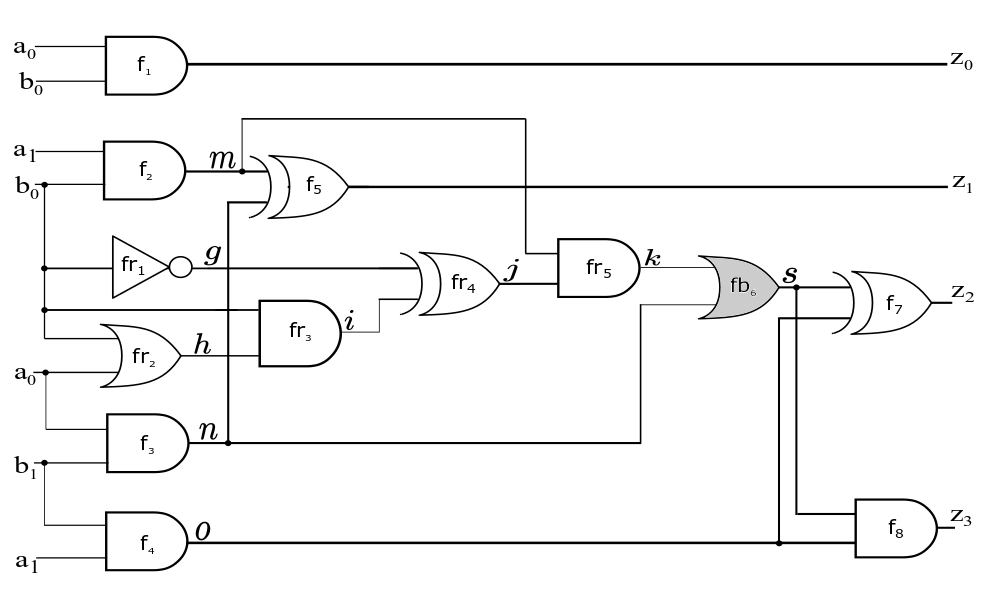
\includegraphics[scale = 0.2]{int_mul_red_b.png}
    \caption{2-bit integer multiplier with a bug at $s$.}
    \label{fig:3mult}
\end{figure}

The \spec is: $f = \sum_{i=0}^{2n-1}
2^iz_i-\sum_{i=0}^{n-1} 2^ia_i\cdot \sum_{i=0}^{n-1} 2^ib_i$.
Verification is done by performing \Grobner Basis reduction, $f
\xrightarrow{J+J_0}_+r$. We find $r = -4\cdot a_0\cdot a_1\cdot
b_0\cdot b_1+4\cdot a_0\cdot b_1$. Since $r \neq 0$, verification
detects the presence of a bug in the design. We will now attempt to
rectify the circuit at an internal net (single-fix
rectification is possible at net $s$ itself!). 
\end{Example}

\section{Computing a rectification function}\label{rect}

%% This paper considers single-fix rectification of integer arithmetic circuits. We define single-fix rectification as follows:

%% \begin{Definition}
%% Single  fix-rectification  at  target  net $x_i$ means  that  there  exists  a  polynomial  function $U(X_{PI})$ which,  when implemented  at  net $x_i$,  ensures  that circuit $C$ correctly implements the specification $f$.
%% \end{Definition}

%% In \cite{utkarsh:fmcad18}, a rectification check theorem (Theorem V.1) was presented to confirm if a net $x_i$ admits single-fix rectification. This rectification check was presented for finite field arithmetic circuits. However, this theorem can be extended to the model used for integer arithmetic circuits. In this paper, we assume that the theorem is applied to a net $x_i$, where single-fix rectification is found to be possible. Given such a net $x_i$, we compute a rectification polynomial which can be implemented at that net to rectify the circuit. 

Assume that post-verification debugging has been performed and a net
$x_i$ in the circuit $C$ has been identified that admits single-fix
rectification. Therefore, our objective is to now compute a function
$x_i = U(X_{PI})$ such that $U: \{0,1\}^{|X_{PI}|}\rightarrow
\{0,1\}$. We will first show how to compute $U$ as a polynomial
function, and then how to synthesize it as a circuit. Polynomially, we
will represent the hitherto unknown component $U$ as $f_i = x_i -
U(X_{PI})$, where $x_i$ is the leading term of the corresponding
polynomial. 


% \subsection{Problem Statement}

% \begin{itemize}
%     \item Given $R = \Q[x_1,\dots,x_n]$.
%     \item Given a word-level specification polynomial $f$.
%     \item Given a buggy $k$-bit integer multiplier circuit $C$. The bit-level primary inputs are $\{a_0,\dots,a_{k-1}\}$ and $\{b_0,\dots,b_{k-1}\}$. The bit-level primary outputs are $\{z_0,\dots,z_{2k-1}\}$.
%     \item Analyze the topology of the circuit and derive RTTO.
%     \item Given a system of polynomial equations modeling the gates in the circuit $C$, $F=\{f_1,\dots,f_s\}\subset R = \Q[x_1,\dots,x_n]$ and the set $F_0=\{x_1^2-x_1,\dots,x_n^2-x_n\}$.
%     \item Given a net $x_i$ which admits single-fix rectification.
% \end{itemize}

% Our goal is to find a polynomial function $x_i = U(X_{PI})$ that maps $\{0,1\}^{|X_{PI}|} \rightarrow \{0,1\}$, such that $f \in \langle f_1,\dots,f_i:x_i-U(X_{PI}),\dots,f_s,x_1^2-x_1,\dots,x_n^2-x_n \rangle$. This polynomial function rectifies the circuit.

%\subsection{Procedure to compute rectification function}

Let $R = \Q[x_1,\dots,x_n]$ and let $F =
\{f_1,\dots,f_i:x_i-U(X_{PI}),\dots,f_s\}$ the system of polynomials
modeling the correct circuit and $U(X_{PI})$ is the unknown
rectification polynomial to be computed. The polynomials are ordered
according to RTTO, s.t. $lt(f_1) > lt(f_2) > \dots > lt(f_i):x_i
> lt(f_{i+1}) > \dots > lt(f_s)$. The desired rectification function
$U(X_{PI})$ computed must satisfy the condition $f \in \langle
f_1,\dots,f_i:x_i-U(X_{PI}),\dots,f_s,x_l^2-x_l \rangle$, where $x_l
\in X_{PI}$. This polynomial function $U(X_{PI})$ can be computed
using the combination of extended \Grobner Basis and ideal membership
testing. As the polynomial $f_i = x_i-U$ corrects the circuit, we can write:
\vspace{-1mm}
\begin{equation}
\label{eq:eqn1}
%\begin{split}
   f \in \langle  f_1,\dots,f_{i-1},\boldsymbol{f_i: x_i - U},f_{i+1},\dots,f_s,  x_l^2-x_l \rangle 
%\end{split}
\end{equation}

The ideal membership relation of $f$ can be written as:
\vspace{-0.5mm}
\begin{equation}
    \label{eq:eqn2}
\begin{split}
f = & h_1f_1 + h_2f_2 + \dots+\boldsymbol{h_if_i}+\dots+h_sf_s \\
& + \sum_{x_l \in X_{PI}} H_l
\cdot(x_l^2-x_l)    
\end{split}
\end{equation}

where $\{h_1,\dots,h_s,H_l\} \subset R$ are arbitrary polynomials. Substituting $f_i = x_i - U$:
\vspace{-1mm}
\begin{equation}
\begin{split}
    f = & h_1f_1 + h_2f_2 + \dots+\boldsymbol{h_i(x_i-U)}+\dots+h_sf_s \\
    & + \sum_{x_l \in X_{PI}} H_l \cdot(x_l^2-x_l)
\end{split}
\end{equation} 
\vspace{-0.25in}

\begin{equation}
\begin{split}
 f = & h_1f_1 + h_2f_2 + \dots+\boldsymbol{h_ix_i-h_iU}+\dots+h_sf_s \\
 & + \sum_{x_l \in X_{PI}} H_l \cdot(x_l^2-x_l)   
\end{split}
\label{eq:eqn3}
\end{equation}

\vspace{-0.15in}

\begin{equation}
\label{eq:eqn4}
\begin{split}
   & f - h_1f_1 - h_2f_2 - \dots-h_ix_i \\
   & = -h_iU+\dots+h_sf_s + \sum_{x_l \in X_{PI}} H_l \cdot(x_l^2-x_l) 
\end{split}
\end{equation}

%\vspace{-0.1in}

Notice that on the L.H.S. of Eqn. (\ref{eq:eqn4}), the polynomials
$f, f_1,\dots,f_{i-1}$ and the monomial $x_i$ are known polynomial expressions. Therefore, $f$ can be divided by $f_1,\dots,f_{i-1}$ and $x_i$ to obtain the respective quotients of the division
$h_1,\dots,h_i$ and remainder $r$. The polynomial $f$ can be written as 
\begin{equation}
f = h_1f_1 + h_2f_2 + \dots + h_ix_i + r
\end{equation}
The remainder $r$ can be computed as:
\begin{equation}
r = f - h_1f_1 - h_2f_2 - \dots - h_ix_i
\label{eq:eqnr}
\end{equation}

After $h_i$ is computed (as quotient of division by $x_i$),
the R.H.S. of Eqn. (\ref{eq:eqn4}) consists of $h_i,f_{i+1},\dots,f_s$ and polynomials $x_l^2-x_l$ as known expressions. This
implies:
\vspace{-1mm}
\begin{equation}
f - h_1f_1 - \dots-h_ix_i \in \langle -h_i,f_{i+1},\dots,f_s,  x_l^2-x_l\rangle
\end{equation}
\vspace{-4mm}
\begin{equation}
r \in \langle -h_i,f_{i+1},\dots,f_s,  x_l^2-x_l\rangle
\label{eq:eqn5}
\end{equation}

Note that RTTO renders the polynomial $f_{i+1},\dots,f_s$ a \Grobner
Basis. However, $\{-h_i,f_{i+1},\dots,f_s\}$ is not. We compute its a
\Grobner Basis $G = \{g_1,\dots, g_t\}$. We apply the extended
\Grobner Basis theory explained in Eqn. (\ref{eqn:imt_orig}) to $G$ to
find the ideal membership relation of $r$. 

\vspace{-0.15in}

\begin{equation}
    r = -h_i'h_i+h_{i+1}'f_{i+1}+\dots+h_s'f_s+ \sum_{x_l \in X_{PI}} H_l' (x_l^2-x_l)
    \label{eq:eqn6}
\end{equation}

Then $h_i'$ is a polynomial that satisfies the ideal membership
relation in Eqn. (\ref{eq:eqn1}). According to \cite{utkarsh:fmcad18},
the polynomial $h_i' = U$  rectifies the circuit such that the circuit
matches the specification.   

However, in our model, $h_i'$ is computed over the field of
rational numbers $\Q$. This polynomial may have fractional
coefficients and it may also evaluate to any non-Boolean value in $\Q$
for some primary input vectors. We use the example of a 3-bit
multiplier shown in Fig. \ref{fig:3appmult} to explain this in more
detail.  

\begin{figure}[H]
    \centering
    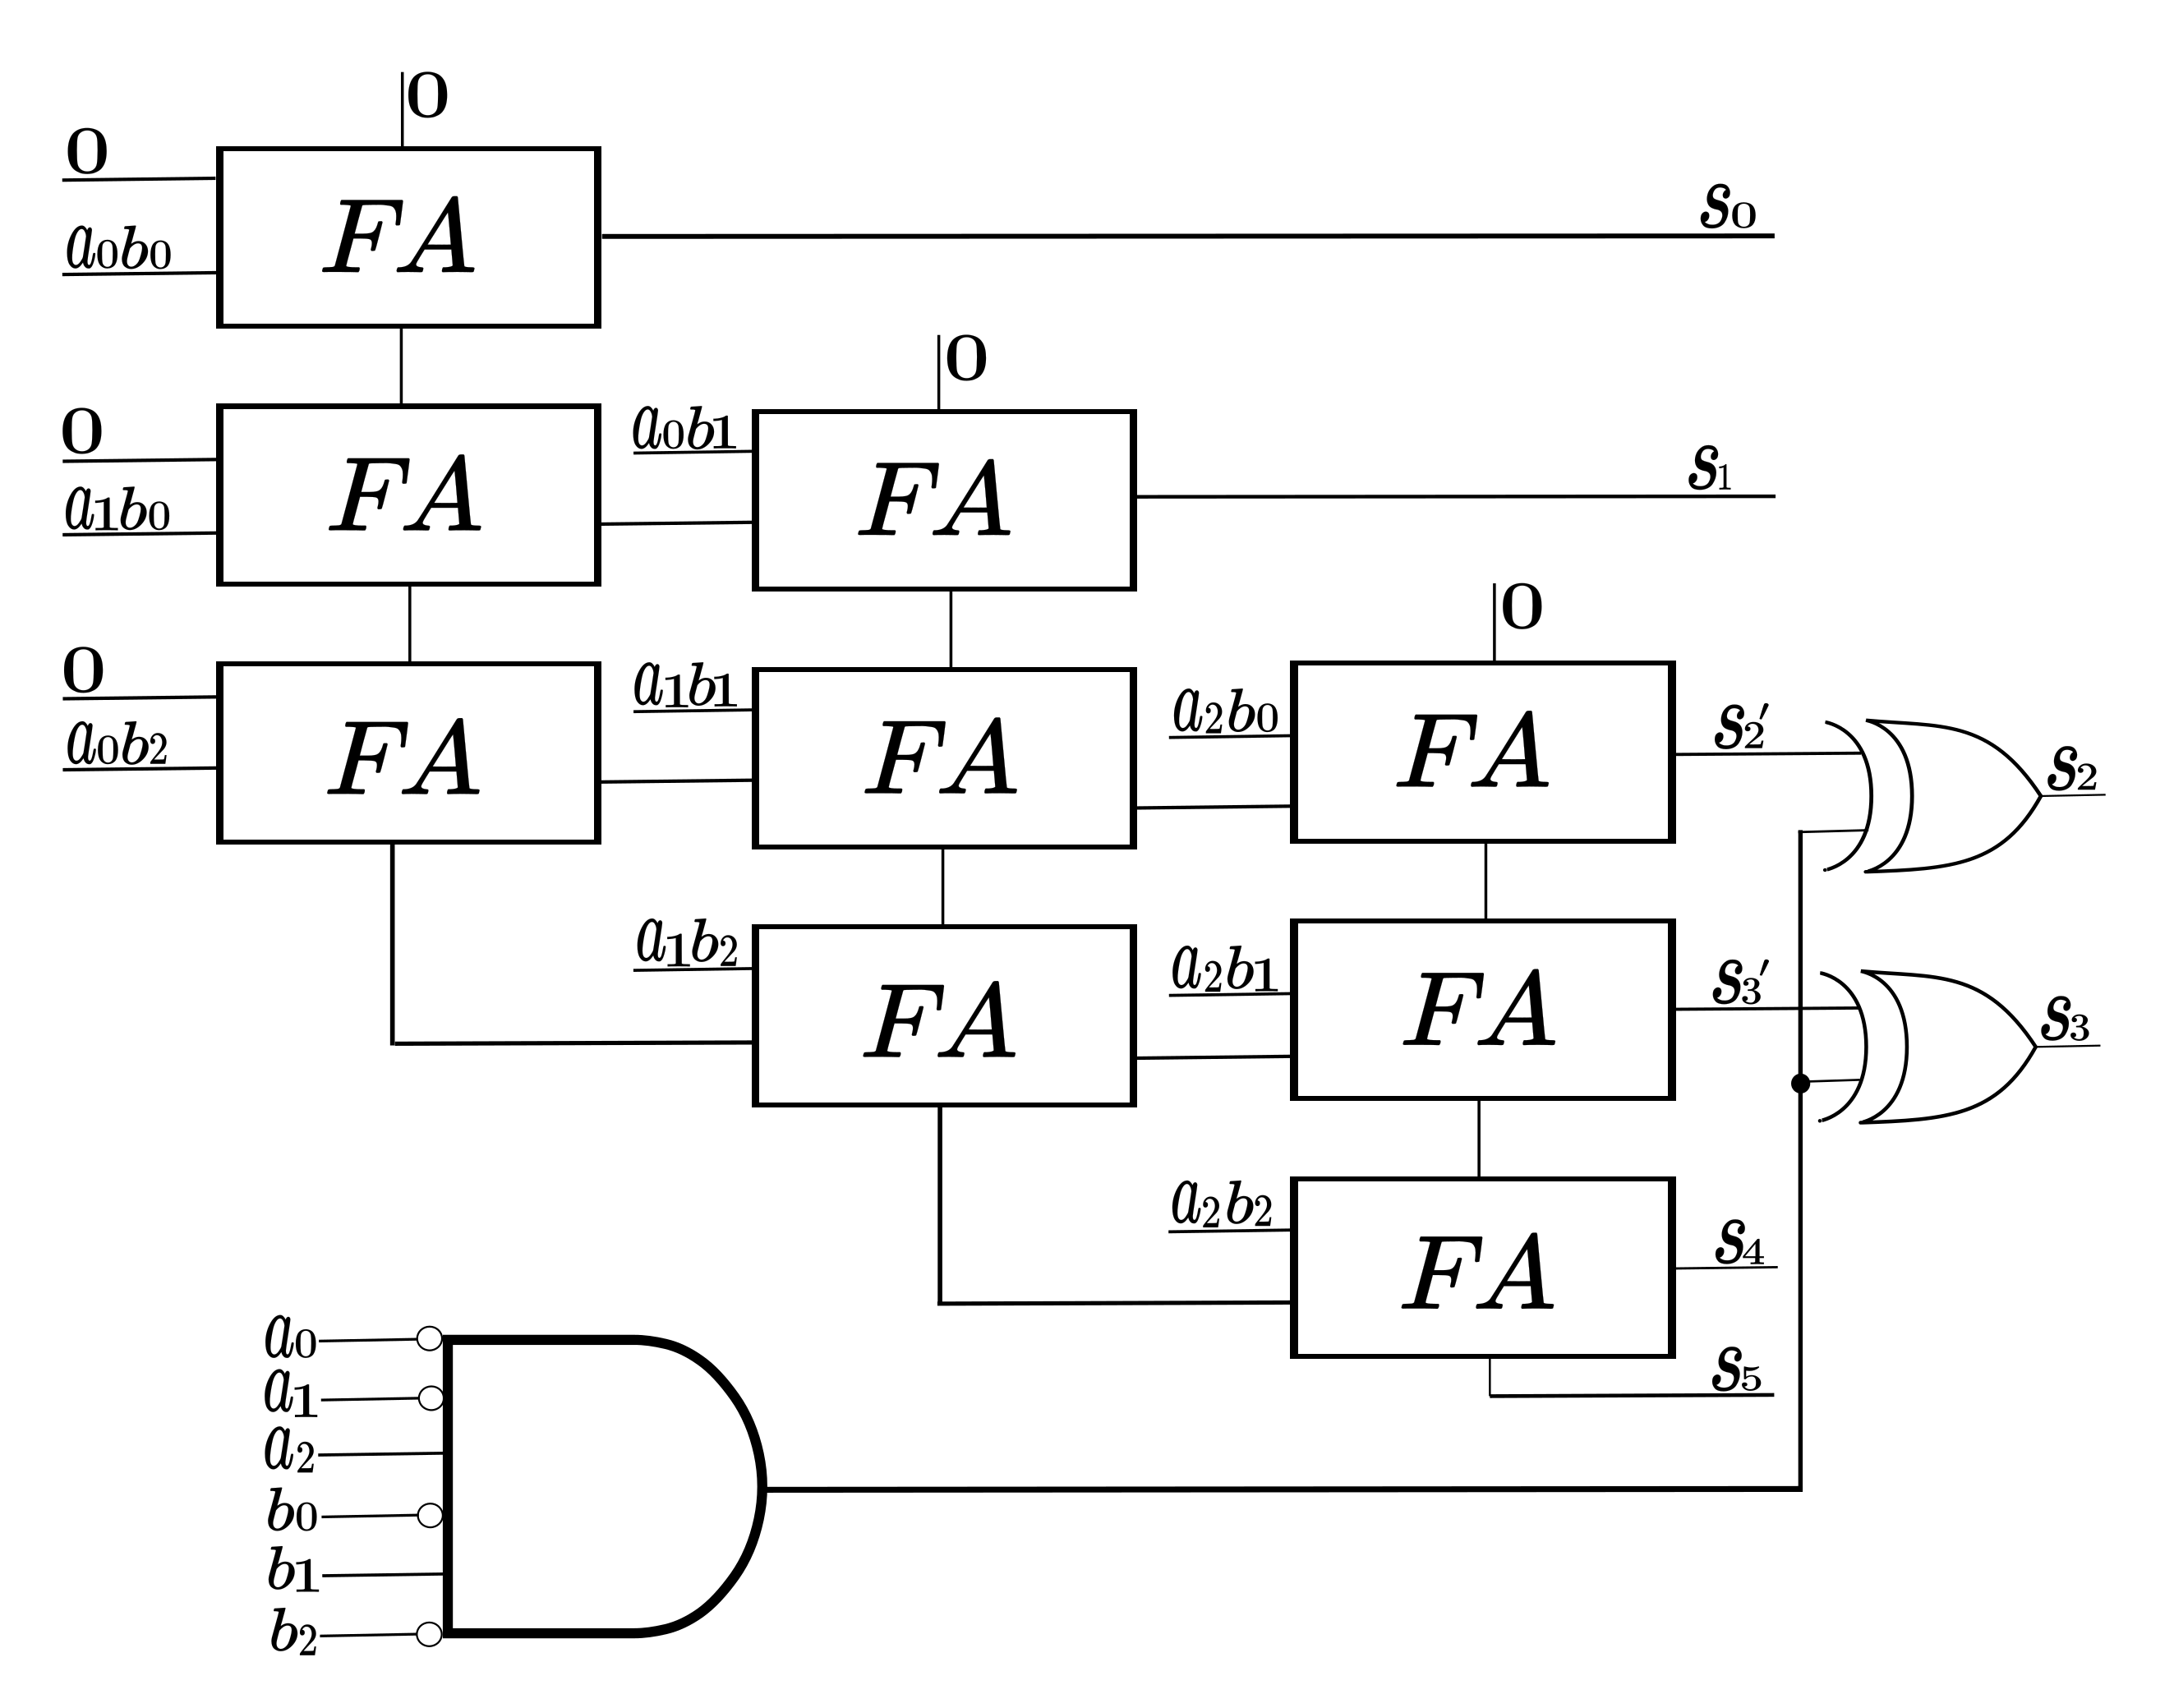
\includegraphics[scale = 0.06]{3appmult.png}
    \caption{3-bit multiplier with additional circuit to introduce a bug}
    \label{fig:3appmult}
\end{figure}

\begin{Example}
The Fig. \ref{fig:3appmult} shows a 3-bit array multiplier circuit. A
bug in introduced in the circuit in the form of additional gates as
shown. Gates are added to the circuit to modify the function of the
circuit at two output bits for one input pattern
$(a_0,a_1,a_2,b_0,b_1,b_2)=(0,0,1,0,1,0)$. Single-fix
rectification is feasible at a net $n_{22}$ in the 
circuit. We apply Eqns. (\ref{eq:eqn1}) to (\ref{eq:eqn6}) and compute
the rectification function $h_i'$, as well as $h_i$, as shown in
Eqn. (\ref{eq:eqn4}).  
{\small
\begin{equation}
    \begin{split}
h_i & = 8\cdot a_0\cdot a_1\cdot a_2\cdot b_0
+16\cdot a_0\cdot a_1\cdot a_2\cdot b_1
-12\cdot a_0\cdot a_1 \\
& -8\cdot a_0\cdot a_2\cdot b_0 
 -16\cdot a_0\cdot a_2\cdot b_1 
 +12\cdot a_0-8\cdot a_1\cdot a_2\cdot b_0 \\
& -16\cdot a_1\cdot a_2\cdot b_1 
+12\cdot a_1+8\cdot a_2\cdot b_0
+16\cdot a_2\cdot b_1
-12        
    \end{split}
    \nonumber
\end{equation}

\begin{equation}
    \begin{split}
h_i' = & -\frac{44}{3}\cdot a_0\cdot a_1\cdot a_2\cdot b_0\cdot b_1\cdot b_2+
\frac{4}{3}\cdot a_0\cdot a_1\cdot a_2\cdot b_0\cdot b_1 \\
& +8\cdot a_0\cdot a_1\cdot a_2\cdot b_0\cdot b_2
+\frac{8}{3}\cdot a_0\cdot a_1\cdot a_2\cdot b_1\cdot b_2 \\
& +\frac{4}{3} \cdot a_0\cdot a_1\cdot b_0\cdot b_1\cdot b_2
-\frac{2}{3}\cdot a_0\cdot a_1\cdot b_0\cdot b_1 \\
&+\frac{4}{3}\cdot a_0\cdot a_1\cdot b_1\cdot b_2
+\frac{8}{3}\cdot a_0\cdot a_2\cdot b_0\cdot b_1\cdot b_2 \\
& -4\cdot a_0\cdot a_2\cdot b_0\cdot b_2 
+\frac{28}{3}\cdot a_1\cdot a_2\cdot b_0\cdot b_1\cdot b_2 \\
& -\frac{14}{3}\cdot a_1\cdot a_2\cdot b_0\cdot b_1
-\frac{8}{3}\cdot a_1\cdot a_2\cdot b_0\cdot b_2 \\
&-\frac{20}{3}\cdot a_1\cdot a_2\cdot b_1\cdot b_2
+\frac{8}{3}\cdot a_1\cdot a_2\cdot b_1 \\
&-\frac{2}{3}\cdot a_1\cdot b_1 
-\frac{4}{3}\cdot a_1\cdot b_2
+1        
\end{split}
\nonumber
\end{equation}
}

We evaluate the polynomial $h_i$ and $h_i'$ for all primary input patterns. The observations are recorded in the following table. 
\vspace{2mm}
\begin{table}[ht]
    \centering
    \begin{tabular}{|c|c|c|} \hline
      $a_0,a_1,a_2,b_0,b_1,b_2$ & $h_i$ & $h_i'$ \\ \hline
       0,0,0,0,0,0 & -12 & 1\\ \hline
       0,0,0,0,0,1 & -12 & 1\\ \hline
       0,0,0,0,1,0 & -12 & 1\\ \hline
       0,1,0,0,0,1 & 0 & $-\frac{1}{3}$\\ \hline
       0,1,0,0,1,0 & 0 & $\frac{1}{3}$\\ \hline
       0,1,0,0,1,1 & 0 & -1 \\ \hline
    \end{tabular}
    \caption{Evaluating $h_i$ and $h_i'$}
    \label{tab:quosol}
\end{table}

In order to conserve space, Table \ref{tab:quosol} shows the data for
only some input patterns.
%We make some observations based on the contents of this table.
The rectification polynomial $h_i'$ has
fractional coefficients. At points where $h_i = 0$, we see that $h_i'$
can evaluate to any value in $\Q$. We found 48 such points where $h_i$
evaluates to 0. At points where $h_i \neq 0$, we always observe that $h_i'$
evaluates to a value in $\{0,1\}$. 
\end{Example}

%Consider the polynomial $h_i$ which is computed as a quotient of
%division by $x_i$ in Eqn. (\ref{eq:eqn4}). We can see that the
%rectification polynomial $h_i'$ depends on the polynomial $h_i$. This
%is also confirmed by the data shown in Table \ref{tab:quosol}.
In order to understand the conditions under which the rectification
polynomial $h_i'$ computes to only Boolean values, we investigate at the
variety of $h_i$. We make the following claims:

%% Let us assume there exists a polynomial $U$, which
%% can be implemented at net $x_i$ to rectify the circuit. This
%% polynomial is a Boolean polynomial, which performs the mapping
%% $\{0,1\}^{|X_j|} \rightarrow \{0,1\}$, where $X_j$ is the set of
%% variable that are less than $x_i$ in RTTO. This polynomial can be
%% reduced to the primary input variables, $U(X_{PI})$. The existence of
%% such a polynomial can be confirmed by performing the rectification
%% check at $x_i$, shown in \cite{utkarsh:fmcad18}.  
%% % \vspace{2mm}

%% Based on these assumptions, 

\begin{Fact}
The polynomials $h_i$ and $h_i'$ are computed in terms of variables in
the set $X_j$, where $X_j < x_i$ in RTTO.  
\end{Fact}

We use \Grobner basis division to compute $h_i$. This division is
shown in Eqn. (\ref{eq:eqn4}). The order of division under RTTO
ensures that $h_i$ is a polynomial in those variables which are less
than $x_i$ in the term order. Similarly, the extended \Grobner basis
algorithm used to compute $h_i'$ in Eqn. (\ref{eq:eqn6}),
ensures that $h_i'$ is a polynomial in those variables which are less
than $x_i$ in the term order. 


%% \begin{Fact}
%% The polynomial $h_i'$ is computed in terms of variables in the set $X_j$, where $X_j < x_i$ in RTTO. 
%% \end{Fact}

\begin{Fact}
{\small 
  \begin{equation}
    h_i(U-h_i') = \sum_{j = i+1}^{s} (h_j-h_j')f_j+\sum_{x_l\in X_{PI}}(H_l-H_l')(x_l^2-x_l)
    \label{eq:eqn7}
\end{equation}
}
\end{Fact}

We get Eqn. (\ref{eq:eqn7}) by combining Eqns. (\ref{eq:eqn4}), (\ref{eq:eqnr}) and (\ref{eq:eqn6}).

\begin{Fact}
  Let $p \in \{0,1\}^{|X_{PI}|}$ be an assignment to the primary
  inputs of $C$. Let $p'$ be the assignment to the all the nets in $C$
  under the application of $p$ to $X_{PI}$; denote $p'|_{X_{PI}} = p$
  as the projection of $p'$ to primary inputs. Then, we have $\forall
  p \in \{0,1\}^{|X_{PI}|},\ \exists p'$, such that $p'|_{X_{PI}} = p$
  and $f_{i+1}(p') = \dots = f_s(p') = 0$. 
\end{Fact}

Clearly, for all primary input assignments, there exists an assignment
to the nets that satisfies all the gates of the circuit. By using the
three facts stated above, we state and prove the following results:

% \begin{Theorem}
% Let point $p \in \{0,1\}^{|X_{PI}|}$ be a point.\\
% (i) If $h_i(p) = 0$, i.e., $p \in V(\langle h_i \rangle + J_0)$, then $h_i'(p)$ evaluates to a value in $\Q$.\\
% (ii) If $h_i(p) \neq 0$, i.e., $p \notin V(\langle h_i \rangle + J_0)$, then $h_i'(p) \in \{0,1\}$.
% \label{thm:quo2}
% \end{Theorem}

\begin{Theorem}
Let there exist a polynomial $U$ that maps from $\{0,1\}^{|X_j|}
\rightarrow \{0,1\}$. Let $p'$ be a point in the affine space such
that $p'|_{X_{PI}} = p$ and $f_{i+1}(p') = \dots = f_s(p') = 0$. If
$h_i(p') \neq 0$, then $h_i'(p) = U(p')$. 
\label{thm:quo}
\end{Theorem}

\textbf{Proof:}
Consider Eqn. (\ref{eq:eqn7}) and point $p'$ such that
$p'|_{X_{PI}}$, and $f_{i+1}(p') = \dots = f_s(p') = 0$. We know that
$x_l^2 = x_l$ at any point $p \in \{0,1\}^{|X_{PI}|}$. Therefore,
R.H.S. of Eqn. (\ref{eq:eqn7}), when evaluated at $p'$, is 0. Then, we
have $h_i(p')(U(p') - h_i'(p')) = 0$.
In L.H.S. of Eqn. (\ref{eq:eqn7}), when $h_i(p') \neq 0$, $U(p') = h_i'(p')$. 

Since we know (or have assumed) that there exists a (Boolean)
rectification function $U$ for $C$ at $x_i$, we know that $U(p')$
evaluates to a value in $\{0,1\}$. Therefore, according to Theorem
\ref{thm:quo}, $h_i'$ evaluates to a Boolean value at those points
where $h_i \neq 0$.  


\begin{Corollary}
Let point $p$ be such that $p \in \{0,1\}^{|X_{PI}|}$. Let $p'$ be a
point such that $p'|_{X_{PI}} = p$. If $h_i(p') = 0$, the polynomial
$h_i'$ can be modified such that $h_i'(p')$ evaluates to a value in
$\{0,1\}$. 
\end{Corollary}

\textbf{Proof:} Consider Eqn. (\ref{eq:eqn7}). Consider a point $p'$ such that $p'|_{X_{PI}}$ and $f_{i+1}(p') = \dots = f_s(p') = 0$. We know that $x_l^2 = x_l$ at any point $p \in \{0,1\}^{|X_{PI}|}$. Therefore, R.H.S. of Eqn. (\ref{eq:eqn7}) is 0.
\begin{equation}
    h_i(U - h_i') = 0. 
    \label{eq:hinot0}
\end{equation}
In L.H.S. of Eqn. (\ref{eq:hinot0}), $h_i(p') = 0$. Therefore, $U$ can
take any value in $\Q$ at $p'$ to satisfy Eqn. (\ref{eq:hinot0}).
%it does not depend on $h_i'(p')$. 

The above results imply that $U(X_{PI})$ evaluate to Boolean values
wherever $h_i(p') \neq 0$, and $U(X_{PI})$ may evaluate to non-Boolean
values in $\Q$ where $h_i(p')=0$. However, ideal membership
Eqn. (\ref{eq:eqn4}) is always satisfied when $h_i(p')=0$
(irrespective of the value of $h_i'(p')$). Hence, we can modify
the polynomial function $h_i'=U$ at those points $p$ where $h_i(p) =
0$, to evaluate to any  value in $\{0,1\}$, without affecting the
ideal membership relation in Eqn (\ref{eq:eqn4}). These points $p$
where $h_i(p)=0$ form the {\it don't care} set for the rectification
function.  

%% Due to the compact structure of arithmetic circuits, we usually
%% compute polynomial $h_i$ such that $V(\langle h_i \rangle + J_0) =
%% \emptyset$. This implies that the polynomial $h_i$ does not evaluate
%% to 0 at any point in $\{0,1\}^{|X_{PI}|}$. 

Based on the above discussion, the following claim can also be easily
shown, and is stated without proof.
\begin{Corollary}
\label{thm:quo2}
If $\forall p \in \{0,1\}^{|X_{PI}|}$ and $h_i(p') \neq 0\ \forall p'$
such that $p'|_{X_{PI}} = p$, then polynomial $U$ is unique and can be
computed as polynomial $h_i'$ using Eqns. (\ref{eq:eqn1})-(\ref{eq:eqn6}).  
\end{Corollary}

%\textbf{Proof:} By extension of proof for Theorem \ref{thm:quo}, $U(p') = h_i'(p'),\ \forall p'$.


{\it Overall Rectification Approach:} i) Compute $h_i$ and $U=h_i'$ as
shown in  Eqns. (\ref{eq:eqn1})-(\ref{eq:eqn6}). ii) Compute $G =
GB(h_i, F_0)$. If $G = \{1\}$, then it implies that $h_i$ has no
zeros, i.e. $h_i(p')\neq 0, \forall p' \in \{0,1\}^n$. Then $U=h_i'$ is a
Boolean function and it can be uniquely computed with integral
coefficients. $U$ can then be reduced $\pmod{ 2}$, where the products
terms can be implemented as AND gates, and sum terms as XOR
gates. iii) If $G = GB(h_i, F_0) \neq \{1\}$, then $h_i$ evaluates to
0 at some points. Evaluate $h_i$ for all points $p'$, and where
$h_i(p')=0$, set $h_i'(p)=U(p)$ as {\it don't cares}, and generate a
function table, which can be synthesized and attached to net $x_i$. 











%% Corollary \ref{thm:quo2} can be explained using the following example of a 2-bit integer multiplier shown in Fig. \ref{fig:3mult}.

%% \begin{figure}[H]
%%     \centering
%%     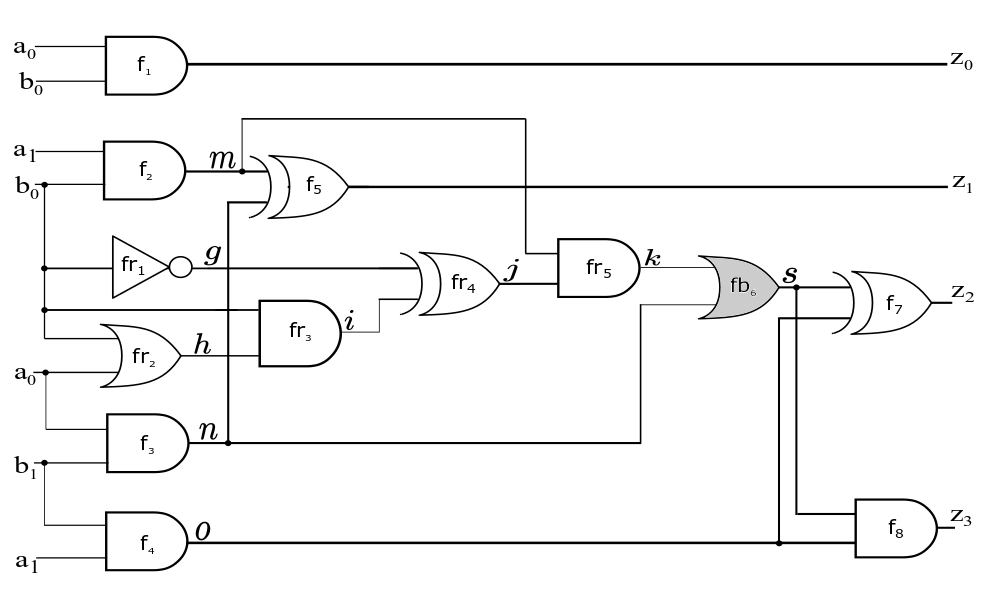
\includegraphics[scale = 0.2]{int_mul_red_b.png}
%%     \caption{2-bit integer multiplier with redundancy with a bug at $s$.}
%%     \label{fig:3mult}
%% \end{figure}
%% \begin{Example}
%% A bug is introduced in the 2-bit integer array multiplier circuit, with added redundancy, shown in Fig. \ref{fig:3mult}. The bug is introduced at a net $s$, which lies in the input cone of the primary outputs $z_2$ and $z_3$. The bug is introduced by replacing the AND gate at $s$ by an OR gate. 



%% \begin{align*}
%% & f_1 = z_0-a_0\cdot b_0 && f_2 = m-a_1\cdot b_0 \\
%% & f_{r1} = g-1+b_0 && f_{r2} = h-a_0-b_0 + a_0\cdot b_0 \\
%% & f_3 = n-a_0\cdot b_1 && f_4 = o-a_1\cdot b_1 \\
%% & f_5 = z_1-m-n+2\cdot m \cdot n && f_{r3} = i-h \cdot b_0 \\
%% & f_{r4} = j-i-g+2 \cdot i \cdot g && f_{r5} = k-j \cdot m \\
%% & \mathbf{f_{b6} = s-k- n+k\cdot n} && f_7 = z_2-s-o+2\cdot s \cdot o \\
%% & f_8 = -z_3+s\cdot o \\
%% \end{align*}

%% The specification for a 2-bit multiplier is:

%% $f = \sum_{i=0}^{2n-1} 2^iz_i-\sum_{i=0}^{n-1} 2^ia_i\cdot \sum_{i=0}^{n-1} 2^ib_i$

%% Verification is done by performing \Grobner Basis reduction, $f \xrightarrow{J+J_0}_+r$.
%% We find $r = -4\cdot a_0\cdot a_1\cdot b_0\cdot b_1+4\cdot a_0\cdot b_1$. Since $r \neq 0$, verification fails and rectification is attempted. Rectification is attempted at net $s$ itself. The procedure to compute a rectification polynomial, shown in Eqns. (\ref{eq:eqn1}) to (\ref{eq:eqn6}), is applied. We compute the following two polynomials. 

%% $$h_i =  4$$

%% \begin{equation}
%% \label{sol}
%% U = a_0\cdot a_1\cdot b_0\cdot b_1
%% \nonumber
%% \end{equation}

%% The polynomial $h_i'$ is the rectification polynomial we computed. The polynomial $h_i = 4$ indicates that it never evaluates to $0$ for any value in $\{0,1\}^{|X_{PI}|}$. Therefore, following Corollary \ref{thm:quo2}, $h_i'$ evaluates to a value in $\{0,1\}$. This is confirmed by evaluating this polynomial for all points in $\{0,1\}^{|X_{PI}|}$. 
%% \label{ex:3bit}
%% \end{Example}

%% The polynomial obtained from our procedure can be synthesized by first reducing it to primary input variables through \Grobner Basis reduction. We compute $U(X_{PI}) \pmod{J+J_0}$. Since this polynomial is a Boolean polynomial, we can find $U(X_{PI}) \pmod{2}$. By interpreting `$+\pmod{2}$' as XOR operation and `$* \pmod{2}$' as AND operation, we can obtain a Reed-Muller form of the rectification function. This AND-XOR expression can be synthesized as a logic circuit by any synthesis tool. 

%% For the rectification polynomial in Example \ref{ex:3bit}, the polynomial was already computed in terms of primary input variables. 

%% The AND-XOR expression for the above rectification function is computed as:

%% $s = a_0\land a_1\land b_0\land b_1$










\vspace{-0.1in}
\section{Experiments}
\label{sec:exp}

We have performed experiments on buggy integer array multiplier circuits. We generated AIG files of array multipliers up to 64 bits by using the \textit{gen -m} command from ABC \cite{ABC}. The tool from the authors in \cite{Armin2017ColumnWiseVO} was used to input obtain *.SING files for the multiplier. We introduced bugs which could be corrected by a single-fix rectification. The complete single-fix rectification procedure is implemented using the SINGULAR symbolic
algebra computation system [ver. 4-1-0][\cite{DGPS_410}]. The experiments
were conducted on a desktop computer with a 3.5GHz Intel
CoreTM i7-4770K Quad-core CPU, 16 GB RAM, running 64-
bit Linux OS. 
\vspace{0.1mm}
\begin{table}[H]
    \centering
    \begin{tabular}{| l | l | l | l | l |}
    \hline
    $k$ & $t_1$ & $t_2$ & $t_3$ & $t_4$ \\ \hline
    %% 2 & 0.002 & 0.003 & 0.007 & 0.005 \\ \hline
    %% 4 & 0.005 & 5.820 & 0.024 & 5.824 \\ \hline
    %% 8 & 0.027 & 9.103 & 0.206 & 9.111 \\ \hline
    %% 12 & 0.120 & 23.137 & 0.641 & 23.158 \\ \hline
    16 & 0.400 & 42.915 & 1.782 & 42.981 \\ \hline
    18 & 0.647 & 48.964 & 2.479 & 49.060  \\ \hline
    28 & 6.329 & 288.448 & 26.707  & 289.860\\ \hline
    32 & 12.119 & 368.319 & 44.965 & 370.579 \\ \hline
    56 & 292.203 & 980.283 & 1221.654 & 1040.504 \\ \hline
    64 & 577.162 & 16.049 & 28.597 & 20.147 \\
    \hline
    \end{tabular}
    \caption{Single-fix rectification of integer multiplier against polynomial specification.}
    \label{tb:tb1}
\end{table}

In the above table, $t_1$ is the time taken to perform verification of the buggy circuits. Times $t_2$ and $t_3$ indicate the time taken to find set of potentially rectifiable nets and identify a net $x_i$ which admits single-fix rectification. The procedure to find potentially rectifiable nets and the rectification target net $x_i$ is borrowed from \cite{utkarsh:fmcad18}. Time $t_4$ is the time taken to compute a rectification polynomial using our approach. 

An interesting observation in Table \ref{tb:tb1} is the difference in
computation time between the 56-bit and 64-bit multiplier. Single-fix
rectification in the 56-bit multiplier is attempted at a net $x_i$
that is located deeper in the circuit, when compared to the placement
of the rectification target in the 64-bit multiplier. This result
shows that the efficiency of our approach depends on the location of
the rectification target net.  

Once we compute a rectification polynomial, we  obtain
an AND-XOR expression for $x_i=U$. We performed experiments to obtain
synthesis results for rectified circuits, compared to the original
correct circuit.   The BLIF files were generated for the
multipliers. The circuit was mapped to a logic library,
\textit{``cadence.genlib1"}, and area-delay stats recorded.
%% , The
%% command \textit{``print\_stats"} was used to obtain area and delay
%% properties of the circuits.


A bug $b_1$ was introduced in the circuit and rectification was
attempted.
%We computed a rectification polynomial and synthesized it
%as a logic circuit. This circuit was used to rectify the bug in the
%original BLIF file.
We then used the command $``resyn"$ in ABC to
re-synthesize the rectified circuit, which was mapped to the
gates in the same logic library. The command \textit{``print\_stats"}
was used to obtain area and delay properties of the rectified
circuit. The above experiment was repeated for other bugs $b_2$ and
$b_3$. The bug $b_2$ is located deeper in the circuit compared to
$b_1$, and bug $b_3$ is located deeper in the circuit compared to
$b_2$. The synthesis results are presented in Table \ref{tb:synth}. 

  \begin{table}
{
%    \centering
%    \resizebox{\textwidth}{!}{
    \begin{tabular}{| c | c | c | c | c | c | c |}
    \hline
    $k$ & \multicolumn{3}{c|}{32} & \multicolumn{3}{c|}{56} \\ \hline
        & $b_1$ & $b_2$ & $b_3$ & $b_1$ & $b_2$ & $b_3$ \\ \hline 
    $area_{(func)}$ & 9 & 41 & 312 & 9 & 87 & TO \\ \hline
   $delay_{(func)}$ & 4.00 & 8.00 & 17.00 & 4.00 & 11.00 & TO \\ \hline     
    $area_{(rect)}$ &  6032 & 6186 & 6469 & 18608 & 18938 & TO \\ \hline     
    $delay_{(rect)}$ & 184.00 & 184.00 & 184.00 & 328.00 & 328.00 & TO \\ \hline  
    $penalty_{(area)}$ & 2.44\% & 5.06 & 9.86\% & 1.30\% & 3.1\% & TO \\ \hline
    $area_{(orig)}$ & \multicolumn{3}{c|}{5888.00} & \multicolumn{3}{c|}{18368.00} \\ \hline 
    
    $delay_{(orig)}$ &  \multicolumn{3}{c|}{184.00} & \multicolumn{3}{c|}{328.00} \\ \hline
    
    \end{tabular}
%}
    \caption{Synthesis Results. $area$ in sq. units. $delay = $ No. of gates.}
    \label{tb:synth}
}
\end{table}


Here, $area_{(func)}$ and $delay_{(func)}$ are the area and delay
numbers for the rectification function; $area_{(rect)}$ and
$delay_{(rect)}$ are the area and delay numbers for the rectified
circuit; $area_{(orig)}$ and $delay_{(orig)}$ are area and delay
numbers for the original correct circuit. In all cases, the
rectified circuit has a larger area compared to the original correct
circuit. Arithmetic circuits are custom designed. However, we are
synthesizing a sub-function to implement in the multiplier circuit and
synthesizing the whole circuit. Logic synthesis for arithmetic
circuits is not very efficient and that is reflected in these results.  

Consider the bug $b_3$ in the 56-bit array multiplier. The bug is
placed in the middle of the circuit and the \Grobner Basis reduction
for verification times out. Therefore, a feasible rectification
polynomial was not computed to rectify this bug. By observing the
results shown in Table \ref{tb:tb1} and Table \ref{tb:synth}, we can
conclude that the location of the bug influences the efficiency of our
approach. One of the limitations of our approach is that we witness
the worst case of the complexity \Grobner Basis reduction based on
the nature/location bugs. 
%
%in case of
%certain bugs, based on their location.  

% Consider the bug $b_3$ in the 56-bit array multiplier. The bug is placed in the middle of the circuit and the \Grobner Basis reduction for verification times out. Therefore, a feasible rectification polynomial was not computed to rectify this bug. By observing the results shown in Table \ref{tb:tb1} and Table \ref{tb:synth}, we can conclude that the location of the bug, and consequently the location of the rectification target, influences the efficiency of our approach. To understand this dependency, we have conducted more experiments on a 16-bit integer multiplier by rectifying various bugs present at different locations in the circuit. 

% We use the column-wise incremental reduction model from \cite{Armin2017ColumnWiseVO} to perform \Grobner Basis reduction in our procedure. This model first divides a $k$-bit integer multiplier into $2k$ slices column-wise.

% Following this model, a $16$-bit integer can be divided into $32$ slices, $C_0$ to $C_{31}$. We introduced a bug in slice $C_2$ at a net located close to the primary output $s_2$. Net $x_i$ is selected so it is also located close to the primary output and admits single-fix rectification. We applied the rectification check, described in Theorem. \ref{thm:rectcheck}, on net $x_i$.  We recorded the time taken to complete the \Grobner Basis reductions required to perform the check. We repeated this procedure for bugs located in the middle of the column structure, as well as for bugs located close to the primary inputs. We repeated these experiments for bugs introduced in other columns, gradually moving towards $C_{31}$. The results of the experiments are shown in Table \ref{tb:t3}. 

% \begin{table}[H]
%     \centering
%         \begin{tabular}{| c | c | c | c |}
%     \hline
%              & NO & NM & NI \\ \hline
%     $C_{2}$  & 2.310 & 2.188 & 2.289 \\ \hline 
%     $C_{4}$  & 3.197 & 2.673 & 2.286 \\ \hline 
%     $C_{6}$  & 202.160 & 26.586 & 2.087 \\ \hline 
%     $C_{10}$ & TO & TO & 2.162 \\ \hline 
%     $C_{12}$ & TO & TO & 2.252 \\
%     \hline
%     \end{tabular}
%     \caption{Time recorded in seconds. Time Out = 10800 seconds.NO = Near Output. NM = Near Middle. NI = Near Input.}
%     \label{tb:t3}
% \end{table}

% The numbers recorded in Table \ref{tb:t3} are the computation time for for applying Theorem \ref{thm:rectcheck} on net $x_i$. The computation times for bugs placed near output (NO), near middle (NM), and near input (NI) are compared. We observe that the \Grobner Basis reductions for rectification check does not complete for bugs placed near the primary outputs in slice $C_{10}$. However, reduction does complete for circuits where the bug is placed close to the primary inputs. The results in Table \ref{tb:t3} indicates that the efficiency of our approach is dependent on the placement of the rectification target net. In cases where the bug is placed close to the primary output, we see the worst case of the complexity of the \Grobner Basis reduction, which is discussed further in the subsequent section. 


\vspace{-0.1in} 
\section{Conclusion}
\label{sec:conclude}

We model the rectification problem using concepts from
algebraic geometry and use symbolic computer algebra algorithms to compute the rectification function $U(X_{PI})$. Using the model presented in \cite{Armin2017ColumnWiseVO}, we obtain a system of polynomials $F = \{f_1,\dots,f_s\}$ to describe the gates of the circuit over the field of rational numbers $\Q$. A net $x_i$ in a buggy circuit is found to admit single-fix rectification, confirming the existence of a polynomial $x_i = U(X_{PI})$ in primary input variables that can rectify the circuit at net $x_i$. The problem of computing $U(X_{PI})$ is modeled as an extended ideal membership testing problem, which is
solved using the \Grobner Basis algorithm. This paper investigates the nature of the rectification function, by stating the conditions under which the rectification polynomial we compute is a Boolean polynomial, i.e., it maps from $\{0,1\}^{|X_{PI}|}\rightarrow \{0,1\}$. We also introduce the concept of don't cares of the rectification function in the computer algebra setup. This paper describes the procedure to synthesize a logic circuit from the rectification polynomial we compute. By conducting experiments on integer array multipliers, we demonstrate the efficiency of our approach. 

%%%%%%%%%%%%%%%%%%%% The bibliography %%%%%%%%%%%%%%%%%%%%%%%%%%%%

\bibliographystyle{IEEEtran}
\bibliography{vikas,utkarsh,tim,xiaojun}

\end{document}

%%%%%%%%%%%%%%%%%%%%%%%%%%%  End of IEEEsample.tex  %%%%%%%%%%%%%%%%%%%%%%%%%%%
